\documentclass[tikz,border=4pt]{standalone}
\usepackage[T1]{fontenc}
\usepackage[scaled=0.95]{helvet}
\renewcommand{\familydefault}{\sfdefault}
\usetikzlibrary{arrows.meta,positioning,calc,patterns}
\definecolor{cA}{HTML}{2a78d6}
\definecolor{cB}{HTML}{eb6834}
\definecolor{cC}{HTML}{1baf7a}
\definecolor{ink2}{HTML}{52514e}
\begin{document}
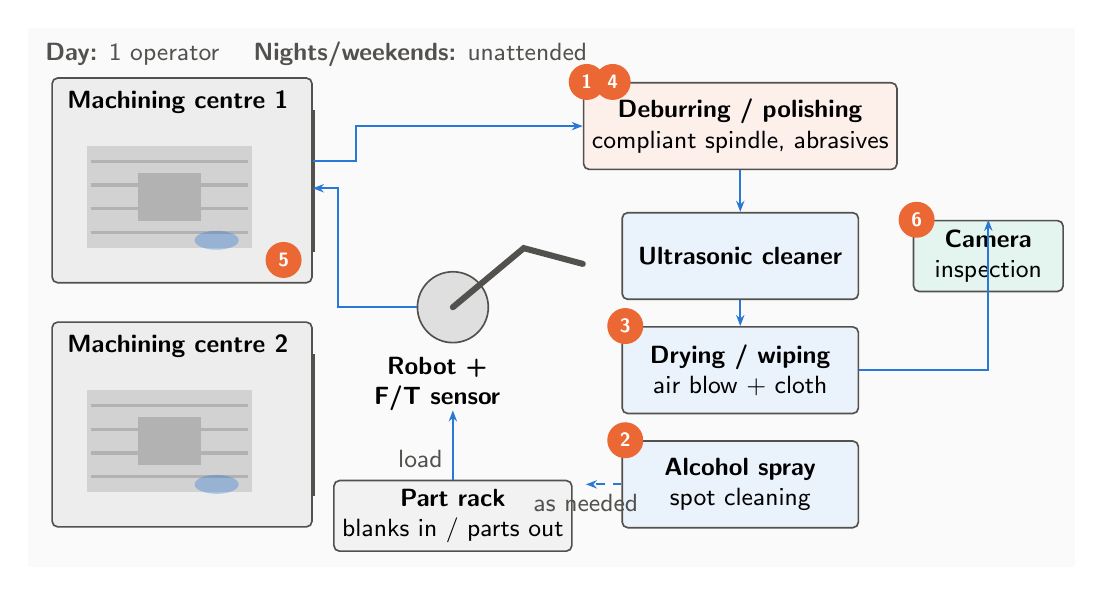
\begin{tikzpicture}[font=\sffamily\small,
  station/.style={draw=ink2, line width=0.6pt, rounded corners=2pt, fill=#1, align=center, inner sep=3pt},
  station/.default={gray!8},
  task/.style={circle, fill=cB, text=white, font=\sffamily\scriptsize\bfseries, inner sep=1.2pt, minimum size=13pt},
  flow/.style={-{Stealth[length=4pt]}, draw=cA, line width=0.7pt},
  lab/.style={text=ink2, align=left}]

% floor
\fill[gray!4] (-0.3,-0.3) rectangle (13.0,6.55);

% machining centres
\foreach \i/\y in {1/3.3, 2/0.2} {
  \node[station=gray!14, minimum width=3.3cm, minimum height=2.6cm, anchor=south west] (mc\i) at (0,\y) {};
  \node[anchor=north west, font=\sffamily\small\bfseries] at ($(mc\i.north west)+(0.08,-0.05)$) {Machining centre \i};
  % table with T-slots
  \fill[gray!35] ($(mc\i.south west)+(0.45,0.45)$) rectangle ($(mc\i.south west)+(2.55,1.75)$);
  \foreach \t in {0.65,0.95,1.25,1.55} \draw[gray!60, line width=1.2pt] ($(mc\i.south west)+(0.5,\t)$) -- ($(mc\i.south west)+(2.5,\t)$);
  \fill[gray!60] ($(mc\i.south west)+(1.1,0.8)$) rectangle ($(mc\i.south west)+(1.9,1.4)$);
  % door
  \draw[ink2, line width=1.6pt] ($(mc\i.south east)+(0,0.4)$) -- ($(mc\i.south east)+(0,2.2)$);
  % coolant on table
  \fill[cA, opacity=0.35] ($(mc\i.south west)+(2.1,0.55)$) ellipse (0.28 and 0.12);
}
\node[task] at ($(mc1.south west)+(2.95,0.3)$) {5};

% robot
\node[circle, draw=ink2, fill=gray!25, minimum size=0.9cm, line width=0.6pt] (rob) at (5.1,3.0) {};
\draw[ink2, line width=2.2pt, line cap=round] (rob.center) -- ++(0.9,0.75) -- ++(0.75,-0.2);
\node[font=\sffamily\small\bfseries, align=center, anchor=north] at ($(rob.south)+(-0.2,-0.05)$) {Robot +\\F/T sensor};

% stations
\node[station=cB!10, minimum width=3.0cm, minimum height=1.1cm] (deb) at (8.75,5.3) {\textbf{Deburring / polishing}\\compliant spindle, abrasives};
\node[task] at ($(deb.north west)+(0.05,0)$) {1};
\node[task] at ($(deb.north west)+(0.38,0)$) {4};

\node[station=cA!10, minimum width=3.0cm, minimum height=1.1cm] (us) at (8.75,3.65) {\textbf{Ultrasonic cleaner}};
\node[station=cA!10, minimum width=3.0cm, minimum height=1.1cm] (dry) at (8.75,2.2) {\textbf{Drying / wiping}\\air blow + cloth};
\node[task] at ($(dry.north west)+(0.05,0)$) {3};
\node[station=cA!10, minimum width=3.0cm, minimum height=1.1cm] (spr) at (8.75,0.75) {\textbf{Alcohol spray}\\spot cleaning};
\node[task] at ($(spr.north west)+(0.05,0)$) {2};

\node[station=cC!12, minimum width=1.9cm, minimum height=0.9cm] (cam) at (11.9,3.65) {\textbf{Camera}\\inspection};
\node[task] at ($(cam.north west)+(0.05,0)$) {6};

\node[station=gray!10, minimum width=2.4cm, minimum height=0.8cm] (rack) at (5.1,0.35) {\textbf{Part rack}\\blanks in / parts out};

% flow arrows
\draw[flow] (rack.north) -- node[lab, left, pos=0.3]{load} ($(rob.south)+(0,-0.85)$);
\draw[flow] (rob.west) -- ++(-1.0,0) |- ($(mc1.east)+(0,-0.1)$);
\draw[flow] ($(mc1.east)+(0,0.25)$) -- ++(0.55,0) |- (deb.west);
\draw[flow] (deb.south) -- (us.north);
\draw[flow] (us.south) -- (dry.north);
\draw[flow] (dry.east) -| (cam.north);
\draw[flow, dashed] (spr.west) -- ++(-0.45,0) node[lab, below, pos=1]{as needed};

% operator / shifts
\node[lab, anchor=north west] at (-0.2,6.5) {\textbf{Day:} 1 operator \quad \textbf{Nights/weekends:} unattended};

\end{tikzpicture}
\end{document}
